\documentclass[11pt]{article}
\usepackage[margin=1.05in]{geometry}
\usepackage{amsmath,amssymb,bm}
\usepackage{booktabs}
\usepackage{siunitx}
\usepackage{tikz}
\usetikzlibrary{arrows.meta,positioning}
\usepackage{listings}
\usepackage{xcolor}
\usepackage[colorlinks=true,linkcolor=blue,citecolor=blue,urlcolor=blue]{hyperref}

\newcommand{\ud}{\,\mathrm{d}}
\newcommand{\vect}[1]{\bm{#1}}
\newcommand{\file}[1]{\texttt{#1}}

\lstset{basicstyle=\ttfamily\footnotesize, frame=single, framesep=4pt,
        backgroundcolor=\color{gray!6}, columns=fullflexible,
        breaklines=true, showstringspaces=false}
\tikzset{
  stage/.style={draw, rounded corners=2pt, align=center, font=\small,
                minimum height=8mm, inner xsep=5pt, fill=purple!6},
  data/.style={draw, align=center, font=\scriptsize\ttfamily, fill=yellow!10,
               minimum height=7mm, inner xsep=4pt},
  fl/.style={-{Stealth[length=2mm]}, thick},
}

\title{Elliptic $\to$ GEO \emph{with} Lunar Gravity: \\
Pipeline, Parameters, and How to Run It}
\author{Michael Casey}
\date{July 26, 2026}

\begin{document}
\maketitle

\begin{abstract}
An operational guide to the CR3BP extension of the elliptic-to-GEO campaign:
the same minimum-fuel transfer, with the Moon's gravity switched on. The
problem formulation, the third-body incorporation and the physical results are
derived and defended at length in the companion note
\file{cr3bp\_geo\_phase1\_note}; this document is deliberately the other half
--- the pipeline, the knobs, how to run a rung or the whole ladder, and where
the numbers land.
\end{abstract}

\tableofcontents

%=======================================================================
\section{What this campaign adds}
%=======================================================================

The two-body campaign (\file{../earth\_elliptic\_to\_geo}) solves the
Haberkorn--Martinon--Gergaud elliptic-to-GEO transfer. This one asks a physical
question of it: \emph{how much does the Moon matter?}

The formulation is unchanged --- modified equinoctial elements, true longitude
as the independent variable, free longitude span $\Delta L$, Bertrand--\'Epenoy
$\varepsilon$-homotopy, trapezoidal collocation in CasADi/IPOPT. What changes
is one opt-in branch in the \emph{shared} right-hand side
\file{lt\_mee\_rhs.m}, which adds the lunar third-body acceleration
\begin{equation}
\vect{a}_{3B} \;=\; -\,\mu_M\!\left[
\frac{\vect{r}-\vect{r}_M}{\|\vect{r}-\vect{r}_M\|^{3}}
\;+\;\frac{\vect{r}_M}{\|\vect{r}_M\|^{3}} \right],
\end{equation}
the second (indirect) term accounting for the acceleration of the Earth-centred
frame itself. The Moon is placed on a circular ephemeris at mean motion $n_M$
with initial phase $\phi_0$. With the perturbation absent the code path is
character-identical to the two-body campaign --- which is the point: the
comparison is like-for-like, and upstream fixes reach this campaign for free.

Two knobs control the physics:
\begin{center}
\begin{tabular}{lll}
\toprule
knob & meaning & range \\
\midrule
\texttt{gain} & lunar mass scale & $0$ (two-body) to $1$ (full Moon) \\
\texttt{phi0} & Moon phase at $t=0$ & $0$ to $2\pi$ \\
\bottomrule
\end{tabular}
\end{center}

\noindent \texttt{gain} is not merely a diagnostic: the solve reaches full
lunar strength by \emph{continuation} in it (\S\ref{sec:pipe}).

%=======================================================================
\section{The pipeline}
\label{sec:pipe}
%=======================================================================

\begin{figure}[htbp]
\centering
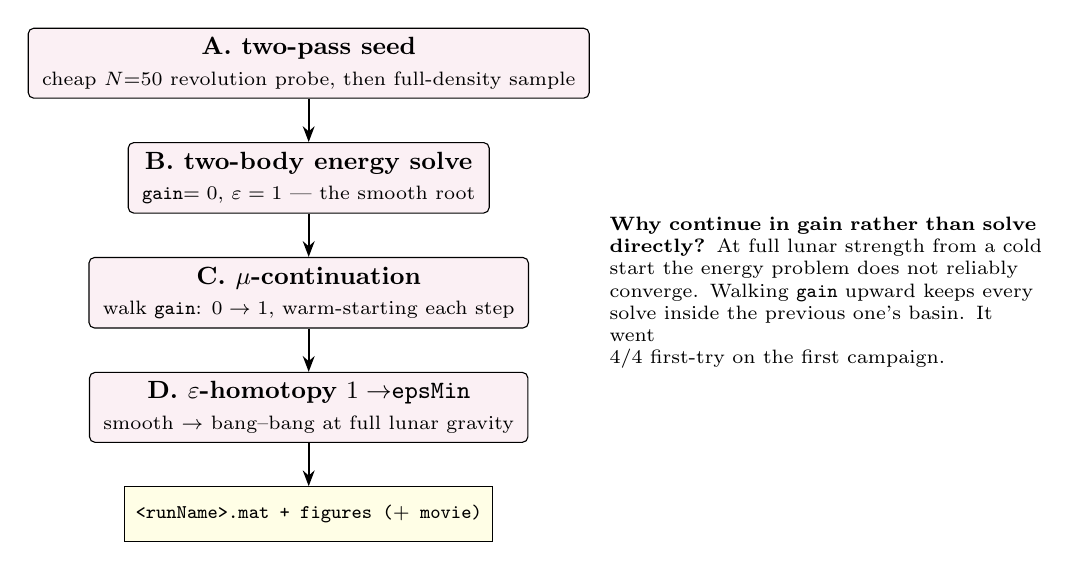
\begin{tikzpicture}[node distance=5.5mm]
  \node[stage] (seed)  {\textbf{A. two-pass seed}\\
        \scriptsize cheap $N{=}50$ revolution probe, then full-density sample};
  \node[stage, below=of seed] (twob) {\textbf{B. two-body energy solve}\\
        \scriptsize \texttt{gain}$=0$, $\varepsilon=1$ --- the smooth root};
  \node[stage, below=of twob] (walk) {\textbf{C. $\mu$-continuation}\\
        \scriptsize walk \texttt{gain}: $0\to1$, warm-starting each step};
  \node[stage, below=of walk] (hom)  {\textbf{D. $\varepsilon$-homotopy} $1\to$\texttt{epsMin}\\
        \scriptsize smooth $\to$ bang--bang at full lunar gravity};
  \node[data,  below=of hom]  (out)  {\file{<runName>.mat} + figures ($+$ movie)};
  \draw[fl] (seed) -- (twob); \draw[fl] (twob) -- (walk);
  \draw[fl] (walk) -- (hom);  \draw[fl] (hom) -- (out);

  \node[right=9mm of walk, font=\scriptsize, align=left, text width=55mm]
      {\textbf{Why continue in gain rather than solve\\ directly?} At full lunar
       strength from a cold\\ start the energy problem does not reliably\\
       converge. Walking \texttt{gain} upward keeps every\\ solve inside the
       previous one's basin. It went\\ 4/4 first-try on the first campaign.};
\end{tikzpicture}
\caption{Stages A--D, all inlined in \file{run\_cr3bp\_geo.m}. Every stage is
gated on \texttt{Solve\_Succeeded} plus defect $<10^{-6}$ and checkpointed
under the run name, so re-invoking resumes.}
\end{figure}

\paragraph{Two implementations, one authoritative.}
\file{bridge\_mu\_continuation.m} and \file{solve\_cr3bp\_minfuel.m} implement
the same sequence as separately callable stages. They produced the Phase-1
development artifacts and are reached today only by \file{verify\_cr3bp\_pmp}
and \file{compare\_vs\_2body}. \textbf{\file{run\_cr3bp\_geo} is the
authoritative pipeline} --- it is what \file{run\_cr3bp\_ladder.sh} drives, so
it produced the certified ladder. Do not assume the two are interchangeable
without checking.

%=======================================================================
\section{How to run it}
%=======================================================================

\begin{lstlisting}[language=Matlab]
cd orbit_transfer/earth_elliptic_to_geo_CR3BP/direct
edit run_cr3bp_geo        % set section 1, then run
\end{lstlisting}

\begin{center}
\begin{tabular}{lll}
\toprule
parameter & meaning & typical \\
\midrule
\texttt{thrustN}    & max thrust [N]; certified anchors at 10/5/2.5/1/0.5/0.2/0.1 & \texttt{5} \\
\texttt{gain}       & lunar mass scale, 0--1                     & \texttt{1} \\
\texttt{phi0}       & Moon phase at $t=0$ [rad]                   & \texttt{0} \\
\texttt{epsMin}     & 1 = min-energy, 0 = min-fuel                & \texttt{0} \\
\texttt{ctf}        & $t_f = c_{t_f}\,t_{f,\min}$                 & \texttt{1.5} \\
\texttt{x0Elems}, \texttt{xfElems} & endpoints ([] = HMG defaults) & \texttt{[]} \\
\texttt{runName}    & basename for every artifact of the run      & --- \\
\texttt{liftDL}     & per-node lifted $\Delta L$ (banded KKT)     & see below \\
\texttt{movieMode}  & render the transfer movie                   & \texttt{false} \\
\bottomrule
\end{tabular}
\end{center}

\begin{lstlisting}[language=bash]
./run_cr3bp_ladder.sh                     # default rungs 5 2.5 1 0.5 0.2 0.1
./run_cr3bp_ladder.sh 1 0.5               # only these
\end{lstlisting}

One MATLAB process per rung (crash isolation), ladder-level resume, and a
failed rung is recorded while the ladder continues.

\paragraph{The deep-rung recipe.} At $\ge\SI{2.5}{\newton}$ the MUMPS
factorization can segfault outright. The cure is \texttt{liftDL} --- replicate
$\Delta L$ per node and tie the copies locally, turning the arrowhead KKT
matrix into a banded one --- together with \texttt{maxIter}$\,\ge4000$. Both
matter: under-iteration silently collapses the deep-$\varepsilon$ tail, so a run
can look converged while its switching structure is unresolved.

%=======================================================================
\section{What the campaign found}
%=======================================================================

\begin{itemize}
\item \textbf{Full certified ladder, \SI{10}{\newton} $\to$
\SI{0.1}{\newton}}, through \file{run\_cr3bp\_geo}.

\item \textbf{The Moon's effect versus thrust.} Roughly \SI{50}{\gram} of
propellant, approximately flat at high thrust, falling to a secular floor near
\SI{30}{\gram} at the deep rungs.

\item \textbf{The Moon's effect versus phase --- and it changes sign.} Sweeping
$\phi_0$ gives $+52$, $-56$, $+69$, $-53$ grams at $0,\pi/2,\pi,3\pi/2$. The
$\pi$-periodicity is the signature of a tidal \emph{quadrupole}: the effect is
not ``the Moon helps'' or ``the Moon hurts'' but a phase-dependent
$\cos 2\phi_0$ structure. Reporting a single number for ``the lunar effect''
without naming the phase would be meaningless.

\item \textbf{First-order optimality: gated.} \textbf{Second-order: not
established}, as everywhere in this repository.
\end{itemize}

%=======================================================================
\section{Where things live}
%=======================================================================

\begin{center}
\begin{tabular}{ll}
\toprule
path & contents \\
\midrule
\file{direct/run\_cr3bp\_geo.m}          & the front door (stages A--D inlined) \\
\file{direct/run\_cr3bp\_ladder.sh}      & the thrust ladder \\
\file{direct/lunar\_params.m}            & Moon constants in canonical units \\
\file{direct/bridge\_mu\_continuation.m}, \file{solve\_cr3bp\_minfuel.m}
                                          & callable stages (Phase-1 path) \\
\file{direct/verify\_cr3bp\_pmp.m}       & PMP verification \\
\file{direct/compare\_vs\_2body.m}, \file{sanity\_bound.m} & analysis \\
\file{direct/viz/}                       & phase sweep, ladder, quad movie \\
\file{doc/cr3bp\_geo\_phase1\_note}      & \textbf{the technical note} (theory, results) \\
\bottomrule
\end{tabular}
\end{center}

\paragraph{The one shared-core edit.} It lives upstream, in
\file{../earth\_elliptic\_to\_geo/direct/core/lt\_mee\_rhs.m}, as the opt-in
\texttt{par.pert} branch. This campaign duplicates nothing else and delegates
its path to the two-body campaign --- the ``extend, don't fork'' pattern that
the repository's 2026-07-26 structure review found had clearly outperformed
both vendoring and forking elsewhere.

\end{document}
